\section{Background}\label{sec:background}

The exponential tendency for data demand predicted by major network providers \cite{cisco2016forecast,kremling2015presentation} is evident. The use of cellular networks for data consumption has become a widespread topic to the general audience. The reason has been the flourishement of online applications services from the last two decades such as:  Whatsapp, Viber (voice and messaging), Facebook, Twitter, Snapchat, Instagram, Google+ (social networking), YouTube, Netflix, SoundCloud, Spotify (video or audio streaming), Google Drive, Dropbox and OneDrive (data storage). Also, these applications have been developed not only for a \ac{PC} but also mobile smartphones and/or tablets that support either the Android, iOS or Windows Mobile \ac{OS}. Hence, it is expected that the data growth will continue within this market. From all these services, streaming applications that are based in multicast scenarios where a transmitter needs to serve tens, hundreds or even thousands of receivers are becoming more frequent in mobile or \ac{WLAN} networks such as \ac{WiFi}. These types of scenarios pose tight requirements in terms of data throughput and delay to ensure a satisfactoring \ac{QoE}.

For the network operator, techniques that can offload the service infrastructure to cope with the data load are needed in order to satisfy this increasing demand. Further, due to network capacity constraints, the end-user might not be connected to a \ac{BS} in a cellular fashion. Instead, the connectivity might be provided by other users either within the cellular spectrum or through a \ac{WLAN}. The deployment of mobile devices without cellular coverage but in a local network can potentially be decentralized. This type of deployment will require the communicating devices to (i) employ multihop communications to ensure connectivity, (ii) use control access mechanisms to avoid interference in the local network. From the devices perspective, energy consumption due to data transmissions has become a limiting factor in terms of battery life. The reason is that mobile devices perform much more internal tasks than older devices from ten years ago. Therefore, mobile network designers need to consider mechanisms and techniques that aim for high throughput and low energy consumption both at the station and the end user devices and that are able to provide data offloading from current network infrastructures.

\subsection{Intra-Session Network Coding for Cooperative Wireless Networks}
The concept of cooperation in wireless network has been investigated before \cite{fitzek2006cooperation,fitzek2007cognitive,heide2012green,fitzek2013implementation,fitzek2013mobile}. The main goal is to diminish the amount of resources allocated (data rate, energy, storage and computational power) to convey an information of common interest from a transmitter to a set of interconnected receivers. The key underlying idea is to split the desired information into pieces and transmit them to the receivers in order for them to share each of their missing pieces. Here, what matters is that the whole information is quickly disseminated into the receivers which aids the \ac{BS} to offload its content. Once this is made, the devices can share data packets by exploiting the short-range commmunications link. Devices connected in this way are called a \textit{mobile cloud} \cite{fitzek2013mobile}. The mobile cloud is a cluster of mobile devices that share resources such as the mentioned before to reduce the usage of them on each device. In this way, mobile clouds allow to improve the overall network performance and user experience.

Introduced by Alshwede et al. \cite{ahlswede2000network}, \ac{NC} appeared as an effective technology to remove the limitations presented previously. In this work, the authors presented a new paradigm for conveying information in communication networks. Instead of following the convention of forwarding data packets from two different data flows, the packets are mixed to create new coded packets. To decode, by receiving a coded packet and knowing the original packets, it is possible to extract the missing information. This key idea let the research community know for the first time that it was possible to code on a \textit{network} basis and not only on a \textit{link} basis as conventional \ac{FEC} technologies do. In the State-of-the-Art, mainly two types of network coding can be identified according to how the packets are mixed from: inter-session network coding and intra session network coding. 

% RLNC and applications

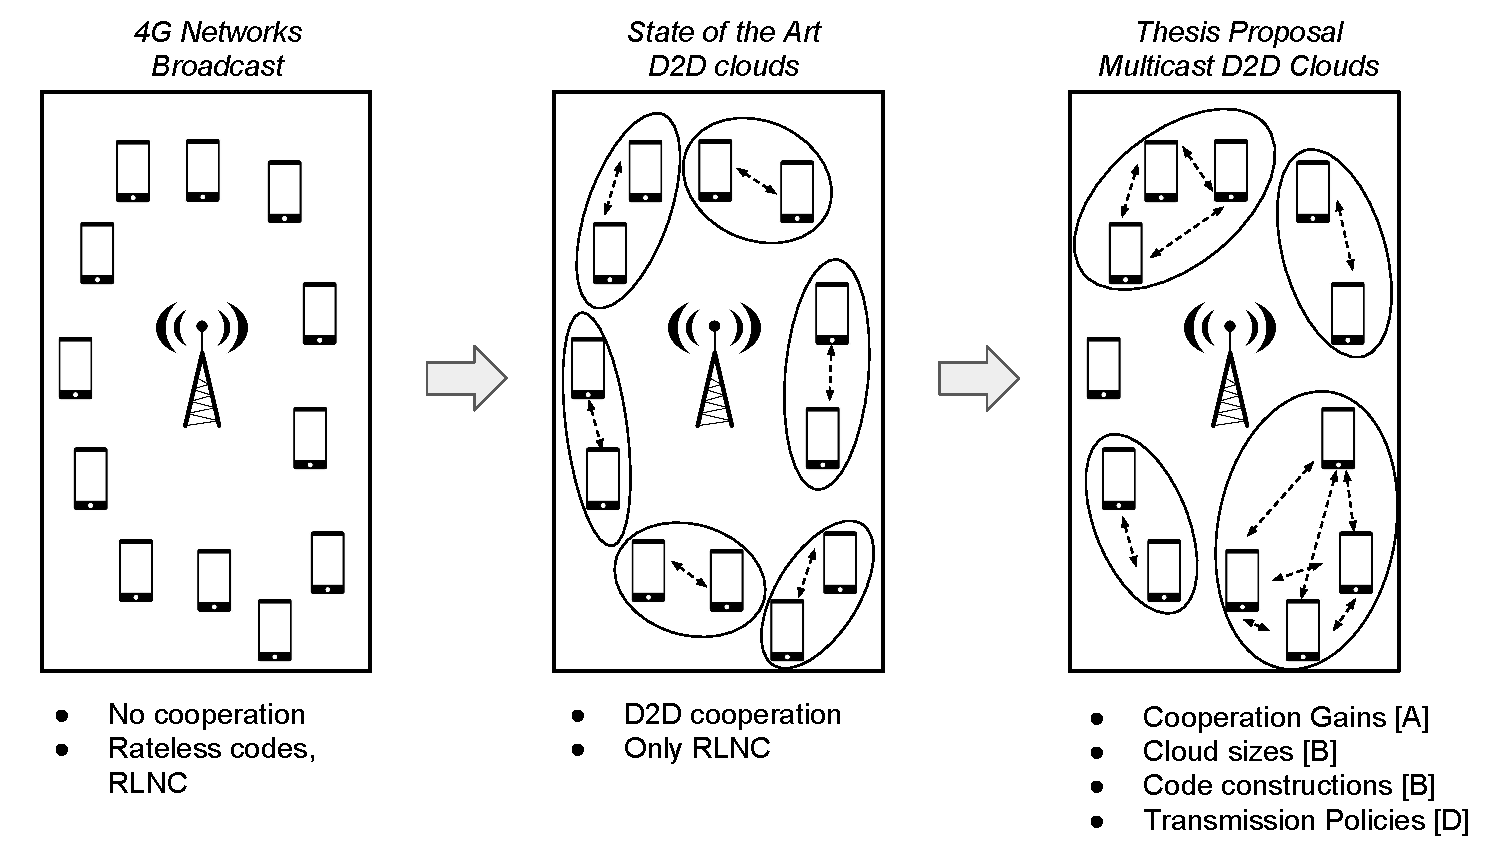
\includegraphics[width=\textwidth]{introduction/figures/thesis-diagrams.pdf}